%!TEX root =../MemoriaTFM.tex
%El anterior comando permite compilar este documento llamando al documento raíz
\chapter{Introducción}\label{chp-01}
\epigraph{You can ask 10 people for a definition of DevOps and likely get 10 different answers.}{Dustin Whittle, 2014\\Developer Advocate at Uber Developer Platform}

\lettrine[lraise=-0.1, lines=2, loversize=0.2]{E}{n} este primer apartado de la memoria se pretende realizar con el lector un recorrido a través del contexto que ha motivado el desarrollo del presente \gls{TFM} para el Máster en Seguridad de la Información y las Comunicaciones  de la Universidad de Sevilla, con el fin de aclarar el objetivo perseguido en su realización. Como conclusión al mismo, se definirá la estructura seguida durante la redacción, introduciendo cada uno de los apartados que se encontrarán a continuación. 

\section{Contexto y motivación}

El año 2017, para empresas englobadas en todo tipo de sectores, está siendo el año de la transformación digital. Estos procesos de transformación exigen distintas formas de trabajo, más ágiles y colaborativas, con las que poder aplicar nuevas tecnologías que permitan conseguir los objetivos del negocio, en entornos que afrontan grandes desafíos culturales, organizativos y operativos e incluso pueden llegar a tener que lidiar con sistemas tecnológicos antiguos y casi obsoletos\cite{expansion2017}. 

Es en este contexto donde el concepto \gls{DevOps} empieza a sonar con más fuerza: el contexto de las metodologías ágiles. 

De esta forma, \gls{DevOps} es un concepto de trabajo, basada en el desarrollo de código, que usa nuevas herramientas y prácticas para reducir la tradicional distancia entre técnicos de programación y de sistemas, respondiendo a la necesidad experimentada por el sector tecnológico de dar una respuesta más rápida a la implementación y operación de aplicaciones. Este nuevo enfoque de colaboración que es \gls{DevOps} permite a los equipos trabajar de forma más cercana, aportando mayor agilidad al negocio y notables incrementos de productividad.

Desde las pruebas de concepto hasta el lanzamiento, pasando por el \textit{testing} y los entornos de prueba, todos los pasos involucrados requieren de la máxima agilidad posible (\autoref{proceso-DevOps}), y eso pasa por integrar los procesos y los equipos de programación con los de sistemas\cite{claranet2017}.

\begin{figure}[htbp]
	\centering
	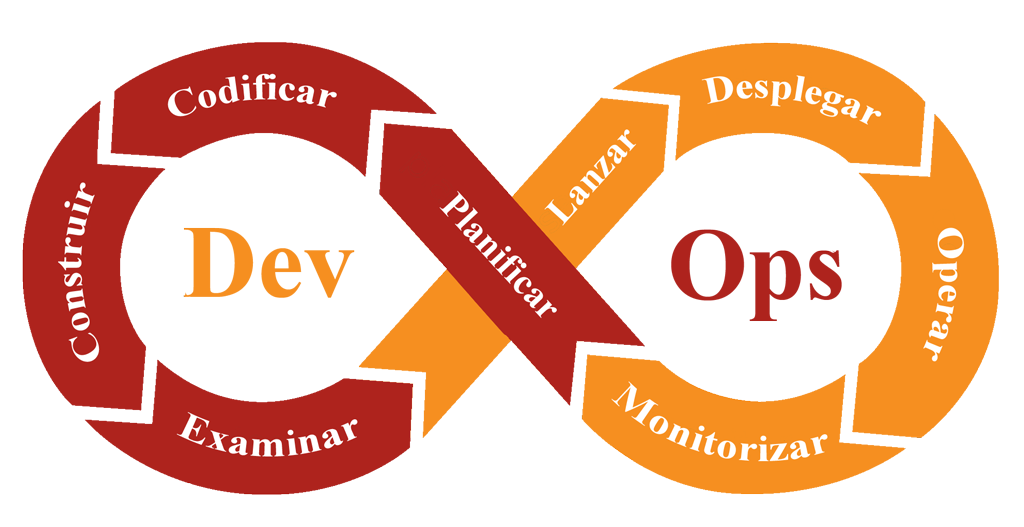
\includegraphics[width=0.80\linewidth]
	{introduccion/figuras/proceso-devops.png}
	\caption{Introducción al proceso DevOps}
	\label{proceso-DevOps}
\end{figure}

Por otro lado, el concepto de contenedor de aplicación (aislamiento de espacio de nombres y gobernanza de recursos) a pesar de no ser un concepto novedoso, está cobrando cada vez más y más relevancia en el panorama de la empresa actual, de la mano de las continuas mejoras que experimentan las tecnologías que lo implementan, simplificando la administración y transformando la forma en que se desarrolla, distribuye y ejecuta el software, en forma de microservicio\footnote{Aproximación para el desarrollo software que consiste en construir una aplicación como un conjunto de pequeños servicios, los cuales se ejecutan en su propio proceso y se comunican con mecanismos ligeros (normalmente una API de recursos HTTP)}, además de proveer la habilidad de encapsular todo el entorno utilizado con el objetivo de ser desplegado en los sistemas de producción de la empresa, manteniendo las mismas características, aumentando la escalabilidad y disminuyendo notablemente los costes asociados a infraestructuras.

Los contenedores juegan un papel clave en un entorno \gls{DevOps} porque soportan las implementaciones de la pila de desarrollo y operaciones completa y van en camino de formar parte de la definición básica de lo que se conocerá como \gls{DevOps} en unos pocos años\cite{searchdatacenter2015}.

Además, la metodología	 \gls{DevOps} representa una gran promesa a la hora de asegurar el desarrollo del software, ya que las organizaciones pueden potencialmente encontrar y remediar las vulnerabilidades con mayor frecuencia y al principio del ciclo de vida de la aplicación, ahorrando costes y tiempo. Conforme al informe de  \textit{"Seguridad de Aplicaciones y DevOps"} de octubre de 2016 promovido por Hewlett Packard Enterprise\cite{hpe2016}, que incluye tanto respuestas cualitativas como cuantitativas de profesionales de operaciones informáticas, líderes de seguridad y desarrolladores, se concluye que el 99\% de los encuestados confirma que la adopción de la cultura \gls{DevOps} aporta la oportunidad de mejorar la seguridad de las aplicaciones. Sin embargo, solo el 20\% realizan análisis de seguridad de aplicaciones durante el desarrollo y el 17\% no utilizan ninguna tecnología que proteja sus aplicaciones, destacando una desconexión significativa entre la percepción y la realidad de la seguridad \gls{DevOps}.

Es en el contexto planteado donde surge la idea del presente \gls{TFM}: aportar mecanismos a la metodología \gls{DevOps} que permitan analizar la seguridad de las aplicaciones desarrolladas y el contenedor que las albergará dentro de la infraestructura de la empresa, sin interferir de manera destructiva con el propio proceso de desarrollo y depliegue de la aplicación.

\section{Objetivo}

El objetivo del presente Trabajo Fin de Máster (\gls{TFM}) es desarrollar un entorno, basado en contenedores, que pueda ser incluido en el proceso de desarrollo e integración continua de la empresa y con el que poder realizar tareas periódicas programadas para analizar estáticamente las posibles vulnerabilidades (\gls{CVE} entre otras) contenidas en las dependencias de aplicaciones desarrolladas mediante los lenguajes de programación Ruby y NodeJS, además de analizar a nivel del \gls{SO} vulnerabilidades presentes en las imágenes que van a constituir el contenedor que dará soporte a dichas aplicaciones.

Como medio para alcanzar el objetivo planteado se va a hacer uso de una serie de aplicaciones y herramientas, entres las que cabe destacar las siguientes, que serán desarrolladas en los próximos apartados:

\begin{itemize}
	\item GitHub\cite{github2017}: Plataforma de desarrollo colaborativo y control de versiones de \gls{SW} donde almacenar, entre otras, el código desarrollado y que será analizadp.
	\item Jenkins\cite{jenkins2017}: Software de Integración Continua (\gls{IC}) con el que automatizar los trabajos periódicos de análisis estático a realizar.
	\item Docker\cite{docker2017}: Proyecto de código abierto que automatiza el despliegue de aplicaciones dentro de contenedores de software, con el que desplegar los distintos elementos requeridos.
\end{itemize}

El trabajo aquí presentado no tiene como objetivo innovar en la tecnología existente, sino por contra valerse de esta para aportar al futuro usuario una herramienta intuitiva y de fácil aplicación, resultado de la agrupación de otras utilidades, con la que poder desplegar con el mínimo esfuerzo el entorno aquí recopilado. 

\section{Estructura de la memoria}


Para facilitar la lectura de la memoria actual, se cree conveniente presentar un resumen de cómo se estructuran los diferentes apartados que contiene.

En el apartado actual, Introducción, se presenta el \gls{TFM} que se va a realizar, aclarando el objetivo perseguido, el contexto en que surge y los aspectos que motivaron su realización.

El apartado \ref{chp-02}, Descripción de la técnica, se pretende dar a conocer, de manera objetiva, las características de la realidad representada, con rasgos tales como elementos que la componen, utilidad, etc. En concreto, el apartado comienza describiendo repasando el panorama actual en las empresas de software. A continuación se ...

El apartado \ref{chp-03}, Entorno de trabajo, está dedicado a conocer las herramientas utilizadas para poder llevar a cabo el desarrollo y la implementación de la parte técnica de este \gls{TFM}.

El apartado \ref{chp-04}, titulado Desarrollo de la aplicación, es el apartado principal de la memoria. En él, se detalla el proceso a seguir durante el desarrollo e implementación de los objetivos presentados en este proyecto, comenzando preparación del entorno que se va a utilizar en el desarrollo, hasta llegar a presentar el Resultado final obtenido.

Por último, el apartado \ref{chp-05}, está dedicado a las Conclusiones y evaluaciones surgidas del proyecto, los objetivos alcanzados y las líneas futuras de trabajo surgidas durante la realización de éste.

\endinput
